\documentclass{article}

\usepackage[spanish]{babel} % Define el idioma del documento

\usepackage[letterpaper,top=4cm]{geometry} % Ajusta el tamaño del papel y las márgenes
\usepackage{graphicx,eso-pic} % Utilizado para insertar imágenes en el encabezado y pie de página
\usepackage{lipsum} % Empleado para generar texto genérico de relleno
\usepackage[style=apa]{biblatex} % Uso de referencias bibliográficas en el estilo APA
\usepackage{csquotes} % Garantiza que los textos citados son compuestos de acuerdo a las reglas del idioma seleccionado
\usepackage{amsmath} % Permite escribir expresiones matemáticas
\usepackage{listings} % Se utiliza para presentar código en fuente monoespacio

\addbibresource{referencias.bib} % Carga el archivo de referencias para ser citado en el cuerpo del documento

% Introduce las imágenes de identidad institucional en el encabezado y pie de página
\AddToShipoutPictureBG{%
  \AtPageUpperLeft{%
    \raisebox{-\height}{
\includegraphics[width=\paperwidth]{img/header_banner.png}}
  }
  \AtPageLowerLeft{%
    \raisebox{1pt}{
\includegraphics[width=\paperwidth]{img/footer_banner.png}}
  }%
}

\begin{document}

%!TEX root = ./documento_unad.tex 
\begin{titlepage}
	\begin{center}
		% \vspace*{0.2cm}
		\Large
		\textbf{CÓDIGO - NOMBRE DEL CURSO}\\
		\vspace{0.5cm}
		% \large
		Unidad X - Etapa Y: Nombre de la Etapa / Fase / Tarea\\
		\vspace{1cm}
		Presentado a:\\
		\vspace{0.3cm}
		\Large
		\textbf{Docente}\\	
		\vspace{0.5cm}

		\vfill

		\large
		Entregado por:\\
		\vspace{0.3cm}
		\Large
		\textbf{Autor 1}\\
		\vspace{0.2cm}
		\large	
		Código: 1.000.000.000\\
		\vspace{0.3cm}
		\Large
		\textbf{Autor 2}\\
		\vspace{0.2cm}
		\large	
		Código: 1.000.000.000\\
		\vspace{0.3cm}
		\Large
		\textbf{Autor 3}\\
		\vspace{0.2cm}
		\large	
		Código: 1.000.000.000\\
		\vspace{0.3cm}
		% \Large
		% \textbf{Autor 4}\\
		% \vspace{0.2cm}
		% \large	
		% Código: 1.000.000.000\\
		% \vspace{0.3cm}
		% \Large
		% \textbf{Autor 5}\\
		% \vspace{0.2cm}
		% \large	
		% Código: 1.000.000.000\\
		\vspace{1cm}

		Grupo: \textbf{123456-123}\\
		\vspace{1.0cm}

		\vfill

		\Large
		\textbf{Universidad Nacional Abierta Y A Distancia - UNAD}\\
		\vspace{0.3cm}
		\large
		\textbf{Escuela De Ciencias Básicas, Tecnología E Ingeniería}\\
		\vspace{0.3cm}
		\textbf{Ciudad}\\
		\vspace{0.3cm}
		\textbf{\today}
		\pagebreak

	\end{center}	
\end{titlepage} % Carga el archivo que define los contenidos de la portada

\tableofcontents % Genera la tabla de contenidos

% Cuerpo del documento, separado en sectiones
\section{Introducción}
Un sistema dinámico es un sistema cuyo estado evoluciona con el tiempo. Los sistemas físicos en situación no estacionaria son ejemplos de sistemas dinámicos, pero también existen modelos económicos, matemáticos y de otros tipos que son sistemas abstractos y, a su vez, sistemas dinámicos. El comportamiento en dicho estado se puede caracterizar determinando los límites del sistema, los elementos y sus relaciones; de esta forma se pueden elaborar modelos que buscan representar la estructura del mismo sistema \cite{albalooshi2003virtual}.
Al definir los límites del sistema se hace, en primer lugar, una selección de aquellos componentes que contribuyan a generar los modos de comportamiento, y luego se determina el espacio donde se llevará a cabo el estudio, omitiendo toda clase de aspectos irrelevantes. 

\lipsum[2-3]

\section{Objetivos}
\begin{itemize}
  \item Utilizar la presentación de espacios de estados para estudiar sistemas dinamicos.
  \item Utilizar software especializado para simular el modelo matemático del sistema físico propuesto.
\end{itemize}

\section{Desarrollo de la Guía}
\begin{enumerate}
  \item Cada estudiante continua con el mismo sistema seleccionado del Anexo 2, tomando como base para este desarrollo el modelo matemático obtenido en el dominio del tiempo en la Etapa 2.
  En la etapa 2 se seleccionó el sistema de suspensión de un automóvil (Fig. \ref{fig:sistema_mecanico}).

  La masa $m_1$ corresponde a la masa de la llanta y su valor corresponde al número de su grupo colaborativo. La masa $m_2$ corresponde a la masa del chasis y es equivalente a su peso corporal en kilogramos. $k_1$ representa la constante elástica de la llanta y su valor corresponde a los 2 primeros números de su documento de identidad. $k_2$ es la constante elástica del resorte de suspensión y su valor corresponde a los 2 últimos números de su documento de identidad. $b_1$ es la constante del amortiguador y su valor corresponde al 5 número de su documento de identidad.

  Se tiene como señal de entrada a $r(t)$ que es el nivel de la calle y la salida es y(t) que representa la posición vertical del chasis del automóvil respecto a algún punto de equilibrio.

  \lipsum[3-4] \cite{sternberg2010dynamical}

  \begin{figure}
    \centering
    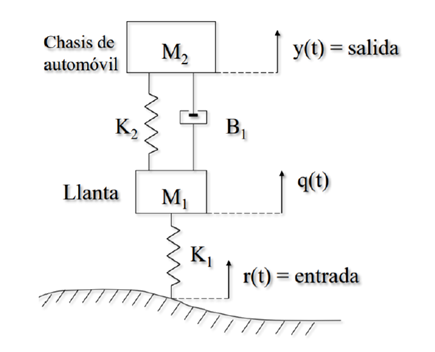
\includegraphics[width=10cm]{img/sistema.png}
    \caption{Sistema mecánico seleccionado.}
    \label{fig:sistema_mecanico}
  \end{figure}

  \item Para el sistema seleccionado, aplicar principios físicos y matemáticos que le permitan obtener el modelo matemático del sistema representado por ecuaciones de espacios de estados.

  Las ecuaciones diferenciales que modelan el sistema en el dominio del tiempo son:

  \begin{align}
    \frac{d^2q}{dt^2} &= \frac{k_1}{m_1}r - \frac{b_1}{m_1}\frac{dq}{dt} - \frac{k_1+k_2}{m_1}q - \frac{b_1}{m_1}\frac{dy}{dt} - \frac{k_2}{m_1}y\\
     \frac{d^2y}{dt^2} &= -\frac{b_1}{m_2}\frac{dy}{dt} - \frac{k_2}{m_2}y + \frac{b_1}{m_2}\frac{dq}{dt} + \frac{k_2}{m_2}q
  \end{align}
  \begin{equation*}
    x_1 = q \quad \Rightarrow \quad \dot{x}_1 = \frac{dq}{dt} \quad \Rightarrow \quad \ddot{x}_1 = \frac{d^2q}{dt^2}
  \end{equation*}
  \begin{equation*}
    x_2 = y \quad \Rightarrow \quad \dot{x}_2 = \frac{dy}{dt} \quad \Rightarrow \quad \ddot{x}_2 = \frac{d^2y}{dt^2}
  \end{equation*}
  \begin{equation*}
    u(t) = r
  \end{equation*}
  \begin{align}
    \ddot{x}_1 &= \frac{k_1}{m_1}u(t) - \frac{b_1}{m_1}\dot{x}_1 - \frac{k_1+k_2}{m_1}x_1 - \frac{b_1}{m_1}\dot{x}_2 - \frac{k_2}{m_1}x_2\\
     \ddot{x}_2 &= -\frac{b_1}{m_2}\dot{x}_2 - \frac{k_2}{m_2}x_2 + \frac{b_1}{m_2}\dot{x}_1 + \frac{k_2}{m_2}x_1
  \end{align}

  \begin{align}
    \begin{bmatrix}
      \dot{x}_1 \\ \dot{x}_2 \\ \dot{x}_3 \\ \dot{x}_4
    \end{bmatrix} =
    \begin{bmatrix}
      0 & 1 & 0 & 0\\
      -\frac{k_1+k_2}{m_1} & -\frac{b_1}{m_1} & -\frac{k_2}{m_1} & -\frac{b_1}{m_1}\\
      0 & 0 & 0 & 1\\
      \frac{k_2}{m_2} & \frac{b_1}{m_2} & -\frac{k_2}{m_2} & -\frac{b_1}{m_2}
    \end{bmatrix}&
    \begin{bmatrix}
      x_1 \\ x_2 \\ x_3 \\ x_4
    \end{bmatrix} + 
    \begin{bmatrix}
      0 \\ \frac{k_1}{m_1} \\ 0 \\ 0
    \end{bmatrix}
    u(t)\\
    y =
    \begin{bmatrix}
      0 & 0 & 1 & 0
    \end{bmatrix}&
    \begin{bmatrix}
      x_1 \\ x_2 \\ x_3 \\ x_4
    \end{bmatrix}
  \end{align}

  \begin{itemize}
    \item $k_1$: dos primeros dígitos de su número de documento de identidad = 80.
    \item $k_2$: dos últimos dígitos de su número de documento de identidad = 69.
    \item $b_1$: quinto número de su documento de identidad = 2.
    \item $m_1$: número grupo colaborativo = 117.
    \item $m_2$: peso corporal en kilogramos = 70.
  \end{itemize}

  \begin{align}
    \begin{bmatrix}
      \dot{x}_1 \\ \dot{x}_2 \\ \dot{x}_3 \\ \dot{x}_4
    \end{bmatrix} =
    \begin{bmatrix}
      0 & 1 & 0 & 0\\
      -\frac{149}{117} & -\frac{2}{117} & -\frac{80}{117} & -\frac{2}{117}\\
      0 & 0 & 0 & 1\\
      \frac{69}{7} & \frac{2}{70} & -\frac{69}{7} & -\frac{2}{70}
    \end{bmatrix}&
    \begin{bmatrix}
      x_1 \\ x_2 \\ x_3 \\ x_4
    \end{bmatrix} + 
    \begin{bmatrix}
      0 \\ \frac{80}{117} \\ 0 \\ 0
    \end{bmatrix}
    u(t)\\
    y =
    \begin{bmatrix}
      0 & 0 & 1 & 0
    \end{bmatrix}&
    \begin{bmatrix}
      x_1 \\ x_2 \\ x_3 \\ x_4
    \end{bmatrix}
  \end{align}

\item Obtener las ecuaciones de espacios de estados y su correlación con la función de transferencia que representa el sistema seleccionado.

\begin{equation*}
  H(s) = C(sI-A)^-1B
\end{equation*}
Donde
\begin{align*}
  A &=
  \begin{bmatrix}
    0 & 1 & 0 & 0\\
    -\frac{149}{117} & -\frac{2}{117} & -\frac{80}{117} & -\frac{2}{117}\\
    0 & 0 & 0 & 1\\
    \frac{69}{7} & \frac{2}{70} & -\frac{69}{7} & -\frac{2}{70}
  \end{bmatrix}\\
  B &= 
  \begin{bmatrix}
    0 \\ \frac{80}{117} \\ 0 \\ 0
  \end{bmatrix}\\
  C &= 
  \begin{bmatrix}
    0 & 0 & 1 & 0
  \end{bmatrix}&
\end{align*}

\begin{align}
  sI-A &= s
  \begin{bmatrix}
    1 & 0 & 0 & 0\\
    0 & 1 & 0 & 0\\
    0 & 0 & 1 & 0\\
    0 & 0 & 0 & 1 
  \end{bmatrix}
  -
  \begin{bmatrix}
    0 & 1 & 0 & 0\\
    -\frac{149}{117} & -\frac{2}{117} & -\frac{80}{117} & -\frac{2}{117}\\
    0 & 0 & 0 & 1\\
    \frac{69}{7} & \frac{2}{70} & -\frac{69}{7} & -\frac{2}{70}
  \end{bmatrix}\\
  &=
  \begin{bmatrix}
    s & -1 & 0 & 0\\
    \frac{149}{117} & s+\frac{2}{117} & \frac{80}{117} & \frac{2}{117}\\
    0 & 0 & s & -1\\
    -\frac{69}{7} & -\frac{2}{70} & \frac{69}{7} & s+\frac{2}{70}
  \end{bmatrix}
\end{align}

Dadas las dimensiones de la matriz, se realizó el resto del desarrollo de manera computacional con MATLAB:

\begin{figure}
\begin{lstlisting}[language=matlab]
clear all
close all
clc
 
k1 = 80;
k2 = 69;
b1 = 2;
m1 = 17;
m2 = 70;
 
A = [0 1 0 0;...
    -(k1+k2)/m1 -b1/m1 -k2/m1 -b1/m1;...
     0 0 0 1;...
     k2/m2 b1/m2 -k2/m2 -b1/m2];
B = [0;k1/m1;0;0];
C = [0 0 1 0];
D = [0];
 
[N,D] = ss2tf(A,B,C,D);
 
H1 = tf(N,D)
\end{lstlisting}
\caption{Código desarrollado usando la representación en variables de estado.}
\end{figure}

\begin{figure}
  \centering
  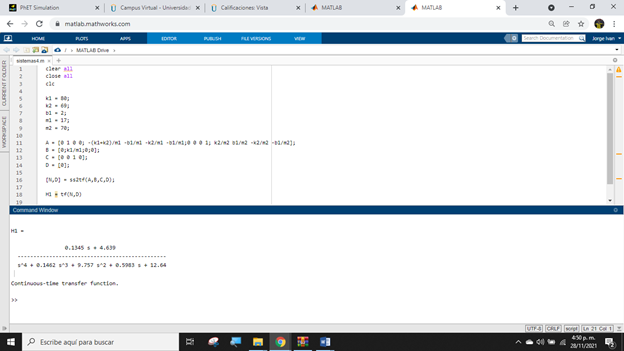
\includegraphics[width=15cm]{img/codigo.png}
  \caption{Ejecución del código desarrollado.}
\end{figure}

\begin{equation*}
  H(s) = \frac{0.1345s + 4.639}{s^4+0.1462s^3+9.757s^2+0.5983s+12.64} 
\end{equation*}

Si comparamos esta ecuación con la obtenida por el método de transformada de Laplace:
\begin{equation*}
  H(s) = \frac{Y(s)}{R(s)} = \frac{(b_1s+k_2)k_1}{(m_2s^2+b_1s+k_2)(m_1s^2+b_1s+k_2+k_1)+(b1_s+k_2)(b_1s+k_2)}
\end{equation*}

\begin{figure}
\begin{lstlisting}[language=matlab]
clear all
close all
clc
 
k1 = 80;
k2 = 69;
b1 = 2;
m1 = 17;
m2 = 70;
 
s=tf('s')
 
num = (b1*s + k2)*k1
den = (m2*s^2 + b1*s + k2)*(m1*s^2 + b1*s + k2 + k1)...
          +(b1*s + k2)*(b1*s + k2)
 
H = num/den
\end{lstlisting}
\caption{Código desarrollado usando la transformada de Laplace.}
\label{fig:códigoLaplace}
\end{figure}

\begin{figure}
  \centering
  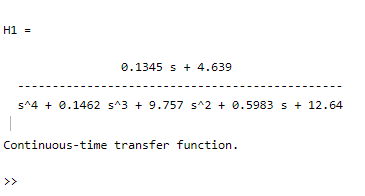
\includegraphics[width=9cm]{img/ecuacion.png}
  \caption{Función de transferencia obtenida.}
  \label{fig:ecuacion}
\end{figure}

Si a la ecuación mostrada en la figura \ref{fig:ecuacion}, dividimos el numerado y el denominador por 10010 obtenemos el resultado mostrado en la figura \ref{fig:ecuacion2}.

\begin{figure}
  \centering
  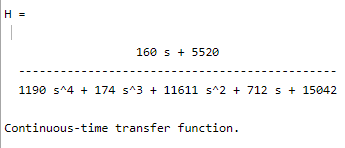
\includegraphics[width=9cm]{img/ecuacion2.png}
  \caption{Función de transferencia normalizada.}
  \label{fig:ecuacion2}
\end{figure}

La ecuación mostrada en la figura \ref{fig:ecuacion2} es igual a la obtenida por espacios de estado, por tanto, el desarrollo es correcto, ahora si calculamos el lugar geométrico de las raíces de este sistema nos encontramos que el sistema tiene 2 polos en el semiplano derecho, por tanto, el sistema es inestable. 

\lipsum[1][1-5]

\item Generar el diagrama de bloques que representa el modelo matemático en espacio de estados del sistema seleccionado, teniendo en cuenta que, una vez transcurridos los 5 primeros segundos, el sistema recibe una señal de perturbación que altera en una unidad la señal de entrada, aumentando así su valor.

En la figura \ref{fig:diagramabloques} se muestra el diagrama de bloques desarrollado en Simulink, usando el bloque \emph{State Space}. En la figura \ref{fig:simulacion} se observan los resultados de ejecutar la simulación para los primeros 10 segundos.

\lipsum[1-2] \cite{WOS:000540232900001}

\begin{figure}
  \centering
  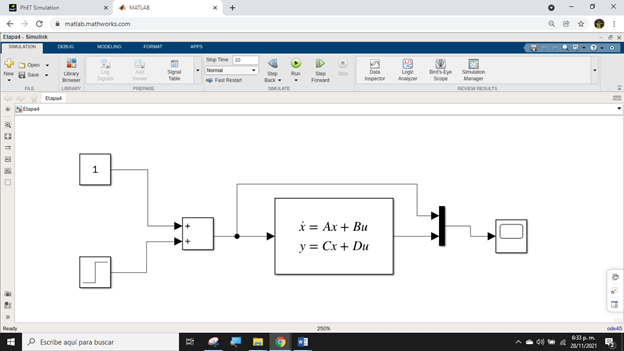
\includegraphics[width=14cm]{img/bloques.png}
  \caption{Diagrama de bloques del sistema diseñado empleando Simulink.}
  \label{fig:diagramabloques}
\end{figure}

\begin{figure}
  \centering
  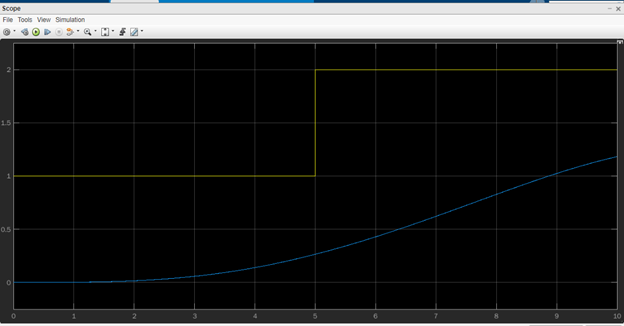
\includegraphics[width=14cm]{img/simulacion.png}
  \caption{Resultados de la simulación del sistema.}
  \label{fig:simulacion}
\end{figure}


\end{enumerate}


\section{Conclusiones}

Representar sistemas dinámicos por medio de espacios de estados es de gran ayuda en el análisis de dichos sistemas, además de dar inicio al control, evalua sistemas físicos en el dominio del tiempo, y junto a Matlab y simulink son de gran ayuda en el estudio de sistemas dinámicos  dado el estudio de las matrices de controlabilidad, como se muestra en \cite{chatterjee2021covid}.

\lipsum[1-2][1-15]

% Genera la bibliografía
\printbibliography[heading=bibintoc]

\end{document}